\documentclass[a4paper]{article}
\usepackage[utf8]{inputenc}
\usepackage[T1]{fontenc}
\usepackage[english]{babel}
\usepackage{amsmath,amsthm,amsfonts,amssymb, mathtools}
\usepackage{mathrsfs}
\usepackage[a4paper,margin=3cm]{geometry}
\usepackage{bm}
\usepackage{siunitx}
\usepackage{tikz}
\usetikzlibrary{calc,arrows,fadings, automata, positioning}
\tikzfading[name=fade inside,inner color=red,outer color=blue]
\usepackage[export]{adjustbox}
\usepackage{graphicx} % ease graphics management

\DeclareMathOperator{\newdiff}{d} % use \dif instead
\newcommand{\dif}{\newdiff\!}
\newcommand{\fdif}[2]{\dfrac{\dif #1}{\dif #2}}
\newcommand{\ffdif}[2]{\dfrac{\dif^2 #1}{\dif #2^2}}
\newcommand{\fndif}[3]{\dfrac{\dif^{#3} #1}{\dif #2^{#3}}}

\newcommand{\fpart}[2]{\dfrac{\partial #1}{\partial #2}}
\newcommand{\ffpart}[2]{\dfrac{\partial^2 #1}{\partial #2^2}}
\newcommand{\fnpart}[3]{\dfrac{\partial^{#3} #1}{\partial #2^{#3}}}

\DeclarePairedDelimiter\abs{\lvert}{\rvert}%
\makeatletter
\let\oldabs\abs
\def\abs{\@ifstar{\oldabs}{\oldabs*}}
\newcommand\norm[1]{\left\lVert#1\right\rVert}

\newcommand{\bhu}{{\bm{\hat{u}}}}

\title{How did the Ever Given get stuck in the Suez canal?}
\author{Miguel De Le Court}
\date{June 2021}

\begin{document}
\maketitle

\vfill

\begin{abstract}
    This reports aims at studying the 2021 Suez canal incident with a 2d CFD model. We start by reconstructing the historical events using a siplified geometry for the canal and the ship. We then formulate an ALE FEM model where the mesh follows the boat in space, and use it to compute the forces on the ship. We then use this data to reproduce the events without enforcing the movements a priori. Based on a slightly tweaked simulation, we show that the incident likely could have been avoided if the ship had been controlled slightly differently. We also point out at the difficulty of finding such ship controls, due to some positive feedback loops that happen when steering the ship.
\end{abstract}
\vfill

\tableofcontents

\newpage
\section{Introduction}
\subsection{Background and Research question}
In March 2021, the Suez Canal was blocked for six days after the Ever Given container ship got stuck sideways in the canal. The Suez canal is route to about 12\% of global trade, and it is estimated that the blockade cost around \$9 Billion per day\cite{bbc:cost}\cite{bbc:cost2}\cite{guardian:cost}. To this day, the effect of the incident are still affecting some parts of the economy\cite{consequ1}\cite{consequ2}, thus, understanding the causes of this incident may be of a crucial importance. 

One known effect that played a significant role in the incident, and which is the most common explaination for it, is the so-called bank effect. When a ship moves forward, an area of high pressure is created around bow of the ship. The water that flows along its sides will, on the contrary, create a low pressure area. When the ship is close to a vertical obstacle, such as the bank, the pressure gradient will produce a couple of forces that will tend to stir the ship\cite{bankeffect}, as shown below. While the bank effect qualitatively explains the movements of the ship around $t=7$ minutes in Figure \ref{fig:snaps}, it is not sufficient to explain what happened previously.


\begin{center}
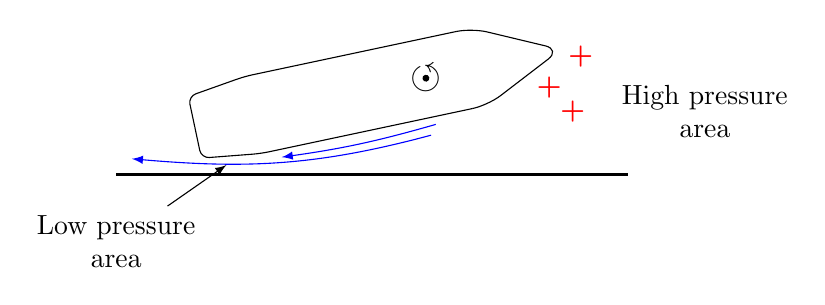
\begin{tikzpicture}
    \begin{scope}[shift={(1,0.6)}, rotate=12, scale=0.5]
        \draw[rounded corners=1mm] (0,0)  -- (0, -0.8) -- (1.5,-1) -- (7,-1);
        \draw[rounded corners=1mm] (0,0)  -- (0, 0.8) -- (1.5,1) -- (7,1);
        \draw[rounded corners=2mm] (7, -1) -- (7.4, -1) -- (9.5, 0) -- (7.4, 1)  -- (7,1);
        \draw [blue, -latex] (6, -1.2) to [bend left=4] (2, -1.2);
        \node at (6,0) (P) {\Large $\circlearrowleft$};
        \fill (6, 0) circle[radius=2.5pt];
    \end{scope}

    \draw[thick] (0,0) -- (6.5,0);
    \draw [blue, -latex] (4,0.5) to[out=195,in=-5] (0.2,0.2);
    \node[red] at (5.5, 1.1) {$\bm{+}$};
    \node[red] at (5.9, 1.5) {$\bm{+}$};
    \node[red] at (5.8, 0.8) {$\bm{+}$};
    \node[right, align=center] at (6.3, 0.8) (nhp) {High pressure\\ area};
    \node[below, align=center] at (0, -0.4) (nlp) {Low pressure\\ area};
    \draw[-latex] (nlp) -- (1.4,0.12);
\end{tikzpicture}    
\end{center}

This project will thus consist in simulating canal obstruction and some other variations on what happened. The goals are to understand why the Ever given got stuck, and what forces were present. We expect to observe and quantify the bank effect at around $t=7$ minutes in Figure \ref{fig:snaps}. We also whish to explain the reasons why the ship got this close to the shore in the first place. With the study of the the typical forces, we also want to highlight possible feedback loops that happen when navigating in a restricted space with a large ship.

\begin{figure}[hbtb]
    \centering
	\includegraphics[width=\textwidth]{Figures/snaps.pdf}
	\caption{Snapshots of the ship positions during the incident}
	\label{fig:snaps}
\end{figure}



\subsection{State of the art}
This project mainly focuses on the study of the fluid forces on a solid, and the interactions that the solid and fluid have. Since the ship will be moving forward during most of the simulation, we will need to move the domain accordingly\footnote{Or use a very large domain for the simulation but this is not the option that was retained.}. These two reasons naturally lead to the choice of using an ALE FEM model that moves along the ship vertically, and deforms to accomodate the rotations and lateral movements. ALE models are commonly used to simulate problems where fluid-structure interaction is of key interest\cite{Jeannette2020Apr}\cite{Wang2018Jul} due to their great interface capturing capabilities. Solids are described in a Lagrangian framework, while the Eulerian framework is most often used for fluids. The solid deformation is computed in a Lagrangian framework and then the mesh is moved using some kind of smoothing that aims at maintaining a reasonable mesh quality for the fluid.  The main challenge with ALE-FEM occurs when large deformations require remeshing to maintain an acceptable mesh quality, or changing the mesh topology. The solution to this problem involves re-meshing globally or locally, and projecting the solution on the new mesh\cite{Remacle2010May}. The main drawbacks of a global remeshing is that the projection of the solution onto the new mesh introduces a lot of numerical diffusion. This also causes problems when we whish to keep a divergence-free field from one mesh to another, as it either adds constraints on the projection, or like in this report, produces unphysical behaviours\footnote{In this context those would be extremely strong pressure gradients.} that may take some time to recover. Another drawback is that a global remeshing is difficult to apply in parallel. Local remeshing like done in \cite{Remacle2010May}, on the other had, requires a rather low level interaction with the mesh generation algorithm, whish was not easyly feasible with dolfin.

\section{Method}
\subsection{Simulation experiments}
This project consists of three experiments. In the first experiment, we are interested in knowing the forces acting on the ship. The conputation will be done by simulating the flow while enforcing the path of the boat through the canal. The forces and torque are then computed base on \eqref{eq:forces} and \eqref{eq:torque}.

The second experiment will try to reproduce the path of the boat, but without enforcing the displacement a-priori, simply by applying the forces computed previously on the boat. In this case, the boat movement is not known a-priori, and the mesh displacement will to be computed based on the forces, together with the fluid motion. 

In the third experiment, we will try to tweak the forces and couples acting on the boat in order to prevent the ship from getting stuck. The goal is to see what king of input would have been necessary to avoid the incident, and evaluate the real world feasability of such inputs.


\subsection{Mathematical model}
The Suez canal incident only involved low speeds, therefore using the incompressible Navier-Stokes equations is a perfectly valid choice. The computation is based on a 2d model of the canal and the ship, with the ship being modelled as a hole in the domain $\Omega$. The boundary conditions on both the ship and the shore are non-slip boundary conditions, with Neumann boundary conditions on the river. The resulting equations inside the domain are thus are thus

\[
    \begin{cases}
        \Dot{\bm{u}} + (\bm{u}\cdot \nabla) \bm{u} +\nabla p - \Delta \bm{u} = 0 & x \in \Omega \\
        \nabla \cdot \bm{u} = 0  & x \in \Omega\\
    \end{cases}
\]
With boundary conditions
\[
    \begin{cases}
        \bm{u} = 0  & x\in \Gamma_\text{shore} \\
        \bm{u} = \bm{u}_\text{boat} & x\in \Gamma_\text{boat}\\
        pn - \nabla \bm{u} = 0  & x\in \Gamma_\text{canal} \\
    \end{cases}
\]
Where $\Gamma_\text{shore}$ is the portion of the boundary that is on the shore, $\Gamma_\text{canal}$ is the artificial boundary that cuts the canal, and $\Gamma_\text{boat}$ are the areas against the boat. The interaction between the ship and the water is governed the Newton's second law.

\subsection{Numerical model}
For the numerical model, it is more convenient to work in an ALE framework, as it can easily capture both the mesh deformation and displacement. The numerical model will be similar to the one from lab 4, where we seek an approximation $(\bm{u}, p) \in V \times Q$ such that
\[
    \left(\bm{\Dot{u}} + ((\bm{u}-\bm{w}) \cdot \nabla) \bm{u}, \bm{v}\right)_\Omega - (p,\nabla \cdot \bm{v})_\Omega + (\nu \nabla \bm{u},\nabla \bm{v})_\Omega + (\nabla \cdot \bm{u}, q)_\Omega + SD(\bm{u},p;\bm{v},q)_\Omega = 0
\]
for all $(\bm{v}, q) \in V \times Q$, with $SD(\bm{u},p;\bm{v},q)_\Omega$ a stabilisation term. All of the computations will use the non-dimentionnal form of the NSE. The scaling parameters are $U=\SI{6}{m/s}$, $L=\SI{400}{m}$, $\rho = \SI{1000}{kg/m^3}$ and $\mu = 10^{-3}\ \si{Pa\cdot s}$, resulting in a Reynolds number $Re = 2.4 \times 10^{9}$. For the rest of the report, we will denote the dimentionless quantities with a ``hat'' : $\bhu = \bm{u}/U$. 

\subsubsection{Computation of the forces}
We also need to compute the forces and torques on the boat, which are given by
\begin{align}
    \bm{F}(\bm{u}, p)   &= \int_{\Gamma_\text{boat}} \nu \nabla \bm{u} \cdot n - pn = \underbrace{\mu U L_c Re}_{F_0} \cdot \int_{\hat{\Gamma}_\text{boat}} \hat{\nu} \nabla \bhu \cdot n - \hat{p} n = F_0 \bm{\hat{F}}(\bhu, \hat{p}) \label{eq:forces}\\[2mm]
    \bm{\tau}(\bm{u},p) &= \underbrace{\mu U LL_c Re}_{\tau_0} \cdot \int_{\hat{\Gamma}_\text{boat}} \bm{\hat{r}}(\hat{x}) \times (\hat{\nu} \nabla \bhu \cdot n - \hat{p}n) = \tau_0 \bm{\hat{\tau}}(\bhu, \hat{p}) \label{eq:torque}
\end{align}
where $\hat{\nu} = 1/Re$ and $\bm{r}(x) = x - x_p$ with $x_p$ the point around which me compute the torque (the center of mass of the boat). Note that we need to multiply the integrals by the draught $L_c=\SI{14}{m}$ of the ship to get the correct force values.


\subsection{Mesh deformation and remeshing}
The meshes used in this report are generated using gmsh, as Dolfin's mshr had edge cases where the minimum mesh size was an order of magnitude smaler than desired, imposing a costly CFL bound.

The mesh deformation and displacement is handled by an elastic solid model where we prescribe the displacement at the boundaries. The displacement on the outside boundaries (i.e. the canal and the shore) is 0 on  the $x$ direction, and chosen such that the domain is centered around the ship's center of mass in the $y$ direction. The mesh deformation around the ship can be computed based on the displacement and rotation of the ship as a composition of a rotation and translation. The displacement and translation are either known a priori (experiment 1) or computed based on the fluid-solid interactions.


The large mesh deformations will inevitably lead to a degradation in the mesh quality, requiring a remeshing at some point. We implemented tree criteria to chose when to remesh:
\begin{enumerate}
    \item The mesh quality goes below a certain threshold (0.2)
    \item Some of the cells become too large 
    \item A change in the topology of the domain is required.
\end{enumerate}
A change in the topology is required when the boat gets too close to the shore, or moves away from being too close to the shore. When the boat gets close to the shore, we either crop the boat to make sure that there is enough space for 2 cells between the boat and the boundary, or we extrapolate the boat to connect it to the shore. Having 2 cells between the ship and the shore is necessary to keep a divergence-free velocity. These cases are shown in Figure \ref{fig:topology}.

\begin{figure}[hbtb]
    \centering
	\includegraphics[width=0.8\textwidth]{Figures/topology.pdf}
	\caption{3 different scenarios for dealing with the collision: the boat is cropped, the boat is extended, and the boat naturally makes contact with the boundary}
	\label{fig:topology}
\end{figure}

\subsubsection{Projection problem}
After remeshing, we project the solution $\bhu$ onto the new mesh. This projection is done by Dolfin's project method which is orthogonal in the $L_2$ norm, but has the drawback that the projected solution is not divergence-free anymore. This in turn produces extremely strong unphysical oscillations in the pressure for a about 15 iterations, as shown on Figure \ref{fig:remesh}. Fortunately, this number remains constant regardless of $\Delta t$, so the current code computes 15 iterations with $\Delta t = \Delta t_0/15$. During these 15 iterations, the computation of the force is ruined by the pressure gradient, so we estimate the forces by applying an agressive smoothing on the force. Let $\tilde{F}$ be the force that we use and report, and $\hat{F}^\text{comp}$ the dimentionless computed force. then 
\[
    \tilde{F}_{i+1} = (1-w) \cdot \tilde{F}_{i} + w \cdot \hat{F}^\text{comp}
\]
with $w$ very small after a remesh.

\begin{figure}[hbtb]
    \centering
	\includegraphics[width=0.7\textwidth]{Figures/remesh.pdf}
	\caption{Pressure and velocity fields before and after a remesh. The arrow shows the computed fluid force on the ship.}
	\label{fig:remesh}
\end{figure}

\subsection{Enforcing the forces}
For experiments 2 and 3, we have to use the computed forces to move and accelerate the ship accordingly. The connection between the dimentionless force and acceleration can be expressed as
\begin{align*}
    \bm{\hat{F}} &= \dfrac{M_\text{boat}}{M_0} \cdot \fdif{\hat{\bm{v}}}{\hat{t}}, 
    && M_0 = L^2 L_c \rho \\
    \hat{\tau} &= \dfrac{\hat{I} M_\text{boat}}{M_0} \cdot \fdif{\hat{\omega}}{\hat{t}}, 
    &&\hat{I} = \dfrac{1}{\hat{A}} \int_{\hat{\Omega}_\text{boat}} \dif \hat{A} (\hat{x}^2 + \hat{y}^2)
\end{align*}

The movement of the ship is then computed using Crank-Nicolson's method to integrate the acceleration and velocity. This is an implicit method which is solved iteratively together with the nonlinear iterations in the fluid computation. Doing that, however, leads to an unstable scheme, as the forces begin to scillate and diverge. To solve this problem we use a smoothing similar to the one used after a remesh, leading to the following complete scheme:
\begin{align*}
    \hat{v}_{i+1} &= \hat{v}_{i} + \dfrac{\Delta t}{2} \left[(\tilde{F}_i + \tilde{F}_{i+1}) + (\hat{F}_{i}^\text{other} + \hat{F}_{i+1}^\text{other})\right] \\
    \tilde{F}_{i+1} &= (1-w) \cdot \tilde{F}_{i} + w \cdot \hat{F}_{i+1}^\text{comp}
\end{align*}
The typical value of $w$ is 0.5 in the second experiment and 0.2 in the third experiment. $w$ is also massively scaled down after a remesh. The other (external) forces $F^\text{other}$ are split into two components : the engine and the (truely) external forces. The engine force is assumed to be constant and in the direction the ship is heading to. Its magnitude is computed from the average longitudinal drag early in the simulation. The external forces are computed from the first experiment with

\[
    \dfrac{M_\text{boat}}{M_0} \cdot \fdif{\hat{\bm{v}}}{\hat{t}} = \bm{\tilde{F}} + \bm{\hat{F}}^\text{engine} +  \bm{\hat{F}}^\text{extern}
\]

\section{Results}
\subsection{First experiment : looking at the forces}
The smoothed forces from experiment 1 are shown on Figure \ref{fig:forces}\footnote{The plot is in a vector format so we higly recommend that the reader zooms into the pdf to have a better look.}. 
\begin{figure}[hbtb]
    \centering
	\includegraphics[width=1.03\textwidth, center]{Figures/forces.pdf}
	\caption{Comparison between the computed forces and torque and the expeted forces and torque based on the acceleration.}
	\label{fig:forces}
\end{figure}
The solid lines indicate the computes forces, while the dashed lines are the expected forces based on the acceleration. The vertical lines indicate the moments where we do a remesh. The forces have been decomposed into their lateral and longitudinal component relative to the ship. This, among other things allows an easy computation of the mean drag, but il also clearly highlights that the side forces are \emph{significantly} larger than expected. The longitudinal forces, on the other hand roughly align with the acceleration in terms of magnitude if we correct for the drag/engine force. Looking at the expected and measured lateral forces in more detail, in Figure \ref{fig:forces_wrong}, we see that although the general direction of the force match the expectation, the magnitude of the measured force is more than an order of magnitude greater that expected. A similar story happens to the torque, althoug there the computed torque doesn't even have the expected shape.
\begin{figure}[hbtb]
    \centering
	\includegraphics[width=1.03\textwidth, center]{Figures/forces_wrong.pdf}
	\caption{Comparison between the computed forces and torque and 15 times the expeted forces and torque.}
	\label{fig:forces_wrong}
\end{figure}


\subsection{Second experiment : reproducing the events}
While there clearly is a problem in the side forces from experiment 1, we can still use it and assume that there was an insanely high external side force that balanced the fluid forces. In this experiment we start the simulation at around $\hat{t} = 0.5$ to skip out the startup effetcs. Running the experiment results in a fairly similar path to the historical data. A series of snapshots comparing the simulation with the reality is shown on figure \ref{fig:simu_snaps}.
\begin{figure}[hbtb]
    \centering
	\includegraphics[width=1.03\textwidth, center]{Figures/simu_snaps.pdf}
	\caption{Comparison between the enforced path and the path simulated from the fluid forces}
	\label{fig:simu_snaps}
\end{figure}


\subsection{Third experiment : correcting the course}
In light of the force problems, we decided to try to correct the course by only applying a small torque on the ship. When looking at the angular acceleration and inertia, we see that the maximum dimentionless torque has a magnitude of around 0.05, which is why we limited the applied torque to 0.02. Snapshots of the resulting path are shown on Figure \ref{fig:simu_correct_snaps}. We see that we were able to avoid the collision with the shore until at least $\hat{t} = 8$. The simulation was not computed further in time as the external forces from experiment 1 start to be dominated by the contact forces, and it would be unrealistic to add them when there is no contact.

\begin{figure}[hbtb]
    \centering
	\includegraphics[width=1.03\textwidth, center]{Figures/simu_correct_snaps.pdf}
	\caption{Comparison between the enforced path and the path simulated from the fluid forces with and added torque}
	\label{fig:simu_correct_snaps}
\end{figure}


\section{Discussion}
\subsection{The problem of the lateral force}
Before looking at the lateral force, it is worth noting that the longitudinal force is righ about where we expet it to be. During the first part of the simulation, when the ships simply moves forward, the force is surprisingly constant and with a magnitude of $\hat{F} = 0.0375$. Converting this force to a dimentionnal form gives $F \approx \SI{7500}{kN}$ which, at \SI{6}{m/s} translates to \SI{45}{MW} of power. Given that the engine of the ship is capable producing \SI{60}{MW} for a speed of about \SI{12}{m/s}, the \SI{45}{MW} instead of $\approx \SI{15}{MW}$ can be explained by the drag coefficient which is much smaller in reality than in this model. This also shows the correctness of the force computation and rules out an implementation error for the large side force.

While in theory the side force could be explained by external factors such as wind, the computed force would require windspeeds of around \SI{450}{km/h}, which is clearly ruled out by the historical meteorological data. What mostly happens here is that our model is in 2D, which creates a significant difference compared to the reality: in reality, if the pressure is high on one side of the ship, the water can flow from one side to the other below the ship. Here, the only way to do so is for the water to go around the ship. A consequence is that if we force a small lateral displacement, the fluid in the model will respond with a very large pressure. In reality however, such a displacement would correspond to a much lower pressure. The fact that the computed side forces and the expected side forces have the same shape also supports this conclusion. The ship likely experienced strong side winds that made it move, and this lateral movenent translates to too large side forces in the model, but that are still in the right direction.

\subsection{Consequences of the side force problem}
A consequence of these strong lateral forces is that the bank effects have been largely overestimated. The strong side forces also explains why the computed torque is unusable. The computed torque mainly depends on the pressure on the side, and if those are massively increased, the errors in the torque will also be magnifies. 

Another surprising consequence is a strange restriction on the $\Delta t$ used for experiments 2 and 3. In those, we observe that taking a significantly smaller $\Delta t$ resulted in an unstable simulation, contrary to what is expected. this is due to the fact that the computed overestimated fluid forces and external forces have to balance each other out. If we use a smaller $\Delta t$, we will at some point get different values for the side forces, which creates an unbalance and a strong sideways acceleration. This in turn triggers a very high pressure increase resulting in an even more powerfun side acceleration in the other direction, and the computation blow up.

\subsection{Unexpected command to keep the ship on track}
The third experiment showed that with minimal input, it was possible to correct the course of the ship and avoid the collision. The command that leads to the collision being avoided, however, is often very conter-intuitive: when the ship is close to one side of the canal, the ``correct'' way to guide it is to head to that same side of the canal! This is true for a significant part of the simulation, although not at the end, where when the ships heads to the right, we try to counter-steer it to the left. 

One reason that may explain why we were able to correct the ship's course with a relatively small input is that when a ship starts turning, a positive feed back loops kicks in. Due to the inertia of the ship, a low pressure area is created inside of the cure, which tends to turn the ship even more. 

\section{Conclusion}
\subsection{From the experiments}
Unfortunately, the first experiment failed to quantitatively describe the forces and torque at play during the events. However, it still gives a good qualitative description of what happened if we keep in mind that the lateral forces are grossly overestimated. In combination with the second experiment, we can even conclude that the ship was subject to strong side winds, and know the direction of such winds, although not their magnitude.


Experiment 3 showed that is was indeed possible, and even easy to avoid this incident. We were able to correct it even in the context of insanely high lateral forces and torque! One can however make a very good counter-argument, stating that the commands were very unintuitive, but most importantly they were found using knowledge from the future. The sensitivity of the path relative to some small changes in the torque also supports this argument, stating that the ship is not always a stable system, and as such is difficult to control.

\subsection{Future work and possible improvements}
Regarding the last point, an interesting direction moving forward would be to try to find an algorithm that computes a command to keep the ship inside the canal based exclusively on past data.

The other thing that a future work should focus on is obviously the biggest problem of this report : the lateral forces. Here, the most obvious option would be to go for a 3d model. This is, however, a significantly harder problem to handle, as we would have to deal with the air-water moving boundary, and it would also be very expansive in terms of processing power. An alternative to consider would be to model the ship as a porous media, and spend some time tweaking the porosity to get matching results from the expected and computed forces.

The second biggest problem has to do with the remeshing. A very significant improvement cound be done by changing the algorithm to a local mesh refinement/coarsening. This could massively improve the robustness of the code, and give a better insight on the forces just before the collision where the intense remeshing (and therefore smoothing) lowers the relevance of the results.

Finally, using a proper dataset for the historical data might also improve the quality of the results. These simulation use data obtained from the youtube video in \cite{goodvideo}, followed by a cubic spline interpolation. The $C_2$ nature of the cubic spline ensures that the acceleration is continuous, but the transitions trom one regime to the other still tend to disturm the computed forces.



\newpage
\bibliographystyle{IEEEtran}
\bibliography{biblio.bib}

\newpage
\appendix
\section{Structure and usage of the code}
The code is divided in 2 main blocks, one for getting and processing the data from the youtube video\cite{goodvideo} into a usable format, and then the fluid dynamics code which depends on the output of the first part. 

Running the only the fluid dynamics part requires the following packages:
\begin{itemize}
    \item \texttt{numpy}
    \item \texttt{matplotlib}
    \item \texttt{scipy}
    \item \texttt{dolfin} and \texttt{mshr}
    \item \texttt{numba}
    \item \texttt{gmsh}
\end{itemize}
The fluid sim code is in the file \texttt{main.py}, which heavily relies on \texttt{utils.py}. \texttt{utils.py} contains a set of custom functions that render the main file easier to read and understand. \texttt{utils.py} depends on the 3 following files:
\begin{itemize}
    \item \texttt{raw data/smoothpath.csv}
    \item \texttt{raw data/smooth\_hdg.csv}
    \item \texttt{raw data/smooth\_coast.csv}
\end{itemize} 
If one whishes to generate these 3 files, the following additional packages are required:
\begin{itemize}
    \item \texttt{cv2}
    \item \texttt{pillow}
    \item \texttt{pytesseract}
    \item \texttt{xml}
    \item \texttt{parse}
    \item \texttt{codecs}
\end{itemize}
As well as the data file \texttt{raw data/map.xml} (which is an exported OSM map of the suez canal). The code should be run in the following order:

\begin{itemize}
    \item \texttt{raw data/video2frames.py} : this will download the video (if it is not present in the directory) and analyse its frames to produce a list of coordinates of the ship. It will also run an OCR to get the additional data and save it to a file.
    \item \texttt{raw data/coastlineparse.py} : this will parse the XML map file and produce coordinates for the sides of the the canal, and save them. It depends on the previous output for some visualization.
    \item \texttt{raw data/smoother.py} : this file will combine the long lists of coordinates of the ship and the canal to produce a cubic spline or hermite approximation of the path and the coast. It will also rotate and translate the coordinates to have a canal with vertical sides in the straight section. These results are then saved in the 3 \texttt{csv} files used by the fluid sim.
\end{itemize} 


\end{document}
